% ===========================================
As already observed, it follows from a result of Sylvester that semigroups of embedding dimension $2$ have Wilf number equal to $0$. 
In particular, semigroups of embedding dimension $2$ are Wilf semigroups. 
Many other classes are known to consist of Wilf semigroups. This section gives an account of a large number of them.

The theme is rather popular and it is frequent to check a family of numerical semigroups against Wilf's conjecture, whenever that new family of numerical semigroups is investigated for some possibly other reason.
It may well happen that some results are not referred to in this paper. This is far from meaning that I do not consider the ideas involved important.
In a few cases this may be a matter of choice, but most probably it simply means that the results are not part of my very restricted knowledge. For that, I humbly express my apologies both to the authors and the readers.
 
The results are split into several subsections, according to a criterion that seems difficult to explain. It finally just aims at putting results together so that they can be compared with ease.

Most of the families considered are described through at least two combinatorial invariants such as embedding dimension, the multiplicity or the conductor.
Exceptions (besides finite sets) are families that are completely described by using only one invariant among the embedding dimension, the multiplicity or the number of left elements.
 
Inside each subsection several results are mentioned (through precise numbered statements or just in the text) and there are cases in which the most general one is stated as a theorem. In a few cases there are results mentioned in more than one subsection.
 
In the first subsection, there is an emphasis on a particular ingredient used along the proofs of the various results. The ingredient is an inequality involving the type. As illustrations of the results that can be found there, we shall see that semigroups with embedding dimension up to three, almost symmetric numerical semigroups and those semigroups generated by generalized arithmetic sequences are Wilf semigroups. 
 
The second subsection is about families of semigroups (somehow explicitly) given by some sets of generators. The examples therein share the particularity that all the members have negative Eliahou number.

The third subsection refers to numerical semigroups with nonnegative Eliahou number.
 
The fourth subsection is dedicated to constructions that are somehow natural. In fact, only one such construction is given here: dilations of numerical semigroups. This subsection could certainly be filled with other constructions. My choice just reflects the feeling that possible generalizations could be worth exploring.

Then there is a subsection devoted to numerical semigroups of small multiplicity.

The sixth subsection is about results in which the main attention is given to semigroups with large embedding dimension, when compared to the multiplicity.

Next there appears a subsection containing a result involving numerical semigroups with big multiplicities and possibly small embedding dimensions.
 
The eighth subsection is similar to the sixth, but now the results have an emphasis on semigroups with large multiplicity, when compared to the conductor.
 
In ninth subsection there is a result taking into account an invariant not previously considered (at least in a fundamental way, to the best of my knowledge). It is the second smallest primitive, sometimes called the \emph{ratio}.
 
The final subsection is concerned with families of numerical semigroups that can be described using only one combinatorial invariant. 

%%%%%%%%%%
\subsection{The type as an important ingredient}

The following proposition, due to Fröberg, Gottlieb and Haeggkvist, is at the base of some results on Wilf's conjecture. It implies that semigroups whose type is smaller than its embedding dimension are Wilf.

\begin{proposition}[{\cite[Theorem 20]{FroebergGottliebHaeggkvist1987SF-numerical}}]\label{prop:type}
    Let $S$ be a numerical semigroup. Then $\conductoroper(S)\le(\typeoper(S)+1)\left|\leftsoper(S)\right|$.
\end{proposition}

By proving that the type of a numerical semigroup of embedding dimension~$3$ is either~$1$ or~$2$ (\cite[Th.~11]{FroebergGottliebHaeggkvist1987SF-numerical}) and using the fact that $\conductoroper\ge 2\left|\leftsoper\right|$ referred in Section~\ref{sec:notation}, they obtained that numerical semigroups of embedding dimension~$3$ are Wilf, a result that Dobbs and Matthews~\cite[Cor.~2.6]{DobbsMatthews2006} reproved using a different approach.
%
Using Sylvester's result for embedding dimension~$2$ and the fact that~$\mathbb{N}$ is Wilf, the same authors obtained the following result.

\begin{theorem}[{\cite[Th.~20]{FroebergGottliebHaeggkvist1987SF-numerical}, \cite[Th.~2.11]{DobbsMatthews2006}}]\label{th:type<=3}
    Numerical semigroups of embedding dimension smaller than $4$ are Wilf. 
\end{theorem}

Since there is no upper bound for the type of numerical semigroups of embedding dimension bigger than $3$, (see~\cite[pg.~75]{FroebergGottliebHaeggkvist1987SF-numerical}, for an example due to Backelin), Proposition~\ref{prop:type} can not be used to obtain other general results (but can, and has been applied successfully to particular families of semigroups).


A numerical semigroup $S$ is said to be \emph{irreducible} if it cannot be expressed as the intersection of
two numerical semigroups properly containing it.
$S$ is said to be \emph{symmetric} if it is irreducible and $\Frobeniusoper(S)$ is odd and it is said to be \emph{pseudo-symmetric} if it is irreducible and $\Frobeniusoper(S)$ is even.
One could take the following as definition (see~\cite[Cor~4.5]{RosalesGarcia2009Book-Numerical}): $S$ is \emph{symmetric} if and only if $\genusoper(S) = \conductoroper(S)/2$, while $S$ is \emph{pseudo-symmetric} if and only if $\genusoper(S) = (\conductoroper(S)+1)/2$. 

It can be proved as a simple exercise that irreducible numerical semigroups are Wilf. A more involving proof could be to observe that the type of this class of semigroups does not exceed $2$. 
\begin{proposition}[{\cite[Prop.~2.2]{DobbsMatthews2006}}]\label{wilf-particular:irreducible}
    Irreducible numerical semigroups are Wilf.
    
\end{proposition}
The above result was generalized by Marco La Valle in~\cite[Th. 5.5]{Barucci2009}. Before stating this generalization, a further definition is needed.
A numerical semigroup is said to be \emph{almost symmetric} if its genus is the arithmetic mean of its Frobenius number and its type (see~\cite{BarucciFroeberg1997JA-One-dimensional}). %ok (the same as t=(g+1-2n)+1)
It is a class of semigroups that includes the symmetric ones and the pseudo-symmetric. 

\begin{proposition}[{\cite[Th.~5.5]{Barucci2009}}]\label{prop:wilf-almost-symmetric}
	Almost symmetric numerical semigroups are Wilf.
\end{proposition}

As a consequence of Theorem~\ref{th:type<=3} Dobbs and Matthews derived an interesting corollary:
\begin{corollary}[{\cite[Cor~2.7]{DobbsMatthews2006}}]\label{cor:c<4l} 
	If $S$ is a numerical semigroup with $\conductoroper\le 4 \left|\leftsoper\right|$, then $S$ is Wilf.
\end{corollary}

Also making use of Proposition~\ref{prop:type}, Kunz~\cite{Kunz2016SF-type} obtained the following result (for $p$ and $q$ coprime). See also Kunz and Waldi~\cite{KunzWaldi2017JA-deviation} for some other generalizations.

\begin{proposition}[{\cite[Cor.~3.1]{KunzWaldi2017JA-deviation}}]
	Let $S$ be a numerical semigroup with $\embeddingdimensionoper(S)\ge 3$. Let $p$ and $q$ be two distinct primitives of $S$.
	If $g+h\in (p+S)\cup(q+S)$, for any (non necessarily distinct) primitives $g$ and $h$ of $S$, then $\typeoper(S)\le\embeddingdimensionoper(S) - 1$. In particular, $S$ is Wilf.
\end{proposition}

A semigroup generated by a generalized arithmetic sequence is a semigroup of the form $S = \langle m, hm + d, hm + 2d, \ldots, hm + \ell d\rangle$, where $m, d, h, \ell$ are positive integers such that $m\ge 2$, $\gcd(m,d) = 1$ and $\ell \le m-2$. Note that $m$ and $d$ being coprime ensures that $S$ is a numerical semigroup.
For a picture made up from a semigroup generated by a generalized arithmetic sequence with $m= 20, d=9, h=2, \ell=8$, see Figure~\ref{fig:GAS_m20_h4_d9_l6}.
By using a result of Matthews~\cite[Cor.~3.4]{Matthews2005I-integers} that computes the type of a numerical semigroup generated by a generalized arithmetic sequence, Sammartano observed the following:
\begin{proposition}[{\cite[Prop.~20]{Sammartano2012SF-Numerical}}]\label{wilf-particular:generalized-arithmetic}
	Numerical semigroups generated by generalized arithmetic sequences are Wilf.
\end{proposition}

%%%%%%%%%%%%
\subsection{Semigroups given by sets of generators}\label{sec:sgps-given-sets-generators}

Let $G$ be an abelian group. Let $A\subseteq G$ be a non empty finite subset and let $h$ be a positive integer. (For the purpose of this paper the reader may think of the group as being a cyclic group $\mathbb{Z}/m$ and take $h=3$; for more details, see~\cite[Chap.~4]{TaoVu2006Book-Additive}.)

The set $A$ is said to be a \emph{$B_h$ set} if, for all $a_1,\ldots, a_h,b_1,\ldots, b_h\in A$, the equality
\[a_1 + \cdots + a_h = b_1 + \cdots + b_h\]
holds if and only if $(a_1,\ldots, a_h)$ is a permutation of $(b_1,\ldots, b_h)$. 

Let $m,a,b,n\in\mathbb{N}_{>0}$ be such that $n\ge 3$ and 
\[(3m+1)/2\le a< b \le (5m-1)/3.\]

Let $A\subseteq \{a,\ldots,b\}$ be such that $\left| A \right|=n-1$ and $A$ induces a $B_3$ set in $\mathbb{Z}/m$. That such a set exists follows from~\cite[Proposition 3.1]{EliahouFromentin2018SF-misses}. Finally, let 
\[S=\langle \{m\}\cup A\rangle_{4m}.\]

Eliahou and Fromentin proved the following result:
\begin{proposition}[{\cite[Th.~4.1]{EliahouFromentin2018SF-misses}}]\label{prop:misses}
	Let $S=\langle \{m\}\cup A\rangle_{4m}$ be a semigroup as constructed above. Then
$\wilfoper(S)\ge 9$, in particular $S$ is a Wilf semigroup.
\end{proposition}

Let $p$ be an even positive integer, let $\mu=\mu(p) = \frac{p^2}{4}+2p+2$ and let $\gamma=\gamma(p) = 2\mu(p) - \left(\frac{p}{2} +4\right)$. The following holds:

\begin{proposition}[{\cite[Prop.6]{Delgado2018MZ-question}}]\label{prop:S(q)}
	Let $S=S(p)=\langle \mu,\gamma,\gamma+1\rangle_{p\mu}.$ Then
$\wilfoper(S)>0$, in particular, $S$ is a Wilf semigroup.
\end{proposition}

\begin{example}\label{ex:fromentin1}
	Figure~\ref{fig:fromentin1} is a pictorial representation of the numerical semigroup $S(4)$.
	Note that $S(4)$ is of the form $\langle \{m\}\cup A\rangle_{4m}$, with $m=14$ and $A=\{22,23\}$.
%	\thisfloatsetup{floatwidth=.48\hsize,capbesidewidth=sidefil,capposition=beside,capbesideposition=right}
	\begin{figure}[h]
		\begin{center}
			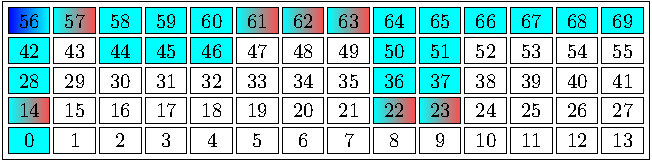
\includegraphics[scale=0.8]{fromentin1.pdf}
		\end{center}
		\caption{Pictorial representation of $S(4)=\langle 14,22,23 \rangle_{56}$. \label{fig:fromentin1}}
	\end{figure} 
\end{example}

To end this subsection I would like to make the following observations:
\begin{remark}\label{rem:non-eliahou}
	The numerical semigroups $S=\langle \{m\}\cup A\rangle_{4m}$ and $S(p)=\langle \mu,\gamma,\gamma+1\rangle_{p\mu}$ defined above have (possibly large) negative Eliahou numbers (see \cite{Delgado2018MZ-question,EliahouFromentin2018SF-misses}). The proof that they are Wilf involves explicit counting.
\end{remark}
\begin{remark}
	The semigroups $\langle \{m\}\cup A\rangle_{4m}$ have depth $4$, while, since the conductor of $S(p)$ is $p\mu$,  there is no bound for the depths of the  semigroups $S(p)$.   
\end{remark}
\begin{remark}
	Several other families obtained using similar constructions to the one in Proposition~\ref{prop:S(q)} can be found in the same paper. In particular, for any given integer $n$,  an infinite family of numerical semigroups with Eliahou number equal to $n$ is obtained.
	All these families consist entirely of Wilf semigroups.
\end{remark}
   
%%%%%%%%%%%
\subsection{Semigroups with nonnegative Eliahou numbers}

Recall that the Eliahou number of a numerical semigroup was introduced in page~\pageref{eq:eliahou-number}. The following result, which states that semigroups with nonnegative Eliahou number are Wilf, appears in~\cite[Prop.~3.11]{Eliahou2018JEMS-Wilfs} (see also~\cite[Cor.~2.3]{EliahouFromentin2018SF-misses}).

\begin{proposition}\label{prop:eliahou-implies-wilf}
	Let $S$ be a numerical semigroup with $\eliahouoper(S)\ge 0$. Then $\wilfoper(S)\ge~0$.
\end{proposition}

This result is similar to Proposition~\ref{prop:type} in the sense that in order to prove that a numerical semigroup is Wilf it suffices to prove that it has nonnegative Eliahou number. The main consequences are referred to in Section~\ref{sec:large-mult}.

While waiting for those consequences, let me refer a result obtained by Eliahou and Marín-Aragón. As they observed, the number $12$ that appears in the statement is the best that can be obtained in this way: Example~\ref{ex:fromentin1} gives a counter example for $\left|\leftsoper\right|= 13$.

\begin{proposition}[\cite{EliahouMarin-Aragon2019}]\label{prop:L<=12}
	If $S$ is a numerical semigroup with $\left|\leftsoper\right|\le 12$, then $S$ has nonnegative Eliahou number and therefore is Wilf. 
\end{proposition}

%%%%%%%%%%%
\subsection{Natural constructions}
Barucci and Strazzanti gave in~\cite{BarucciStrazzanti2018SF-Dilatations} the definition of \emph{dilation of $S$ with respect to $a$}. Namely $D(S,a)=\{0\}\cup \{S+a\mid s\in S\setminus\{0\}\}$. Moreover they proved the following result.
\begin{proposition}[\cite{BarucciStrazzanti2018SF-Dilatations}]\label{prop:dilations}
	If $S$ is a Wilf semigroup $S$ then so is any dilation of $S$.
\end{proposition}

Thus, for each Wilf semigroup $S$, the class $\{D(S,a)\mid a\in S\}$ is an infinite family of Wilf semigroups.

\subsection{Semigroups with small multiplicity}\label{sec:small-multiplicity}
Sammartano~\cite[Cor.~19]{Sammartano2012SF-Numerical} proved that semigroups of multiplicity not greater than $8$ are Wilf. Eliahou~\cite{Eliahou2017-Umea} announced the same kind of result but for multiplicity $12$ (with a similar proof; see the comment just after Theorem~\ref{th:large-embedding-dim-3}). In the meantime, Dhany~\cite[Cor.~4.10]{Dhayni2018PJM-Wilfs} had obtained the result for multiplicity $9$.

A big breakthrough was obtained by Bruns, García-Sánchez and O'Neil, who achieved multiplicity $16$. Their proof involves computational methods, combined with geometrical ones, such as the use of Kunz polytopes.  
\begin{proposition}[\cite{BrunsGarcia-SanchezONeill2019}]\label{prop:mult-16}
	Let $S$ be a numerical semigroup with $\multiplicityoper\le 16$. Then $S$ is Wilf.
\end{proposition}

%%%%%%%%%%%%
\subsection{Semigroups with large embedding dimension (compared to the multiplicity)}\label{sec:large-emb-dim}
As stated in Theorem~\ref{th:type<=3}, numerical semigroups with very small ($\le 3$) embedding dimension are Wilf.
The same happens for those with large embedding dimension (when compared to the multiplicity). 
There are several proofs of the fact that semigroups of maximal embedding dimension (i.e., with embedding dimension equal to the multiplicity). The first one (to the best of my knowledge) is due to Dobbs and Matthews~\cite[Cor.~2.4]{DobbsMatthews2006}.
Sammartano~\cite[Th.~18]{Sammartano2012SF-Numerical}, by means of a rather technical proof involving Apéry sets and the counting in intervals of length $\multiplicityoper$ of elements in the semigroup, proved that numerical semigroups with embedding dimension at least half the multiplicity are Wilf. With refined arguments, 
Dhayni 
(see also her thesis~\cite[Th. 2.3.13]{Dhayni2017phd-Problems}) 
generalized Sammartano's result.

\begin{proposition}[{\cite[Th. 4.12]{Dhayni2018PJM-Wilfs}}]\label{wilf-particular:large-embedding-dim}
    Let $S$ be a numerical semigroup with $\left(2+\frac{1}{\qoper}\right)\embeddingdimensionoper\ge \multiplicityoper$. Then $S$ is Wilf.
\end{proposition}

Eliahou obtained the following impressive generalization by using a graph theoretical approach. The concept of matching (set of independent edges) in a certain graph associated to the Apéry set is used. 

\begin{theorem}[\cite{Eliahou2017-Umea}]\label{th:large-embedding-dim-3}
	Let $S$ be a numerical semigroup with $3\embeddingdimensionoper(S)\ge \multiplicityoper(S)$. Then $S$ is Wilf.
\end{theorem}

%%
\subsubsection*{Some comments}
\begin{enumerate}
    \item Previous result implies that semigroups of multiplicity up to $12$ are Wilf, as already mentioned. 
    Note that a non Wilf semigroup $S$ must satisfy $\embeddingdimensionoper(S)\ge 4$ by Theorem~\ref{th:type<=3}. As it must also satisfy $3\embeddingdimensionoper(S)<\multiplicityoper(S)$, it follows that if $S$ is non Wilf, then $\multiplicityoper(S) > 12$. (Sammartano's result implies $\multiplicityoper(S) > 8$ for $S$ non Wilf.)
    \item A positive answer to Question~\ref{quest:emb-dim-asymptotics} would lead to possibly interesting consequences. For instance, if the limit were $1/2$, one could conclude that asymptotically, as $\genusoper$ grows, half of the numerical semigroups satisfy $3\embeddingdimensionoper\ge \multiplicityoper$, and consequently are Wilf.
\end{enumerate}

Two other simple consequences of Theorem~\ref{th:large-embedding-dim-3} follow. The first is a generalization of a result of Dhany~\cite[Th.~4.9]{Dhayni2018PJM-Wilfs}, who proved that semigroups satisfying $\multiplicityoper-\embeddingdimensionoper\le 5$ are Wilf. At this stage, this remark does not give anything new, but gives a very explicit result.
\begin{remark}
	If $\embeddingdimensionoper(S)\ge\multiplicityoper(S)-10$, then $S$ is Wilf.
\end{remark}
\begin{proof}
	If $\multiplicityoper(S)\le 16$, then Proposition~\ref{prop:mult-16} can be used.
	If $\multiplicityoper(S)\ge 16$, then $\multiplicityoper(S)/3 > 5$. But in this case $\multiplicityoper(S) - 10 \ge \multiplicityoper(S)/3$. In fact, this last inequality is equivalent to $2\multiplicityoper(S) \ge 30$, which holds by hypothesis.
\end{proof}

Another consequence (it suffices Sammartano's result to get it), was observed by Eliahou.
\begin{proposition}[{\cite[Prop.~7.6]{Eliahou2018JEMS-Wilfs}}]
	Let $S$ be a numerical semigroup with $\gcd(\leftsoper\cap \primitivesoper) \ge~2$. Then $S$ is Wilf.
\end{proposition}

%%%%%%%%%%%
\subsection{Semigroups with big multiplicity (and possibly small embedding dimension)}
Moscariello and Sammartano proved that for every fixed value of $\lceil \multiplicityoper/\embeddingdimensionoper\rceil$ the conjecture holds for all values of $\multiplicityoper$ which are sufficiently large and are not divisible by a finite set of primes. Recall from previous subsection that the cases $\lceil \multiplicityoper/\embeddingdimensionoper\rceil\le 3$ have been solved. 
\begin{proposition}[{\cite[Th.~1]{MoscarielloSammartano2015MZ-conjecture}}]\label{prop:very-large-mult}
	Let $S$ be a numerical semigroup. Let $\rho=\big\lceil \frac{\multiplicityoper(S)}{\embeddingdimensionoper(S)}\big\rceil$ and let $\phi$ be the product of prime factors of $\rho$. If $\rho>3$, $\multiplicityoper(S)\ge\frac{\rho(3\rho^2-\rho-4)(3\rho^2-\rho-2)}{8(\rho-2)}$ and $\gcd(\multiplicityoper(S),\phi)=1$, then $S$ is Wilf. 
\end{proposition}
The multiplicities of the semigroups that arise from Proposition~\ref{prop:very-large-mult} are large, as the following \textsf{GAP} session suggests (by showing that for $\rho=4$ the smallest multiplicity is $1680$).
\begin{verbatim}
gap> mult := r -> (r*(3*r^2-r-4)*(3*r^2-r-2))/8*(r-2);
function( r ) ... end
gap> mult(4);
1680
\end{verbatim}

%%%%%%%%%%%
\subsection{Semigroups with large multiplicity (compared to the conductor)}\label{sec:large-mult}
It was proved by Kaplan~\cite[Th.~24]{Kaplan2012JPAA-Counting} that numerical semigroups with conductor not greater than twice the multiplicity are Wilf. This result was generalized by Eliahou. One of the ingredients he used is a theorem of Macaulay on the growth of Hilbert functions of standard graded algebras.
In fact, he proved the following:

\begin{proposition}[{\cite[Th.~6.4]{Eliahou2018JEMS-Wilfs}}]\label{prop:large-mult-Eliahou-jems}
	Let $S$ be a numerical semigroup with $\conductoroper(S)\le 3\multiplicityoper(S)$. Then $S$ has nonnegative Eliahou number.
\end{proposition}
This result combined with Proposition~\ref{prop:eliahou-implies-wilf} leads to the following major fact. (Its importance can be better appreciated by seeing the comments that follow the statement.)

\begin{theorem}[{\cite[Cor.~6.5]{Eliahou2018JEMS-Wilfs}}]\label{th:large-mult-Wilf-jems}
  Let $S$ be a numerical semigroup with $\conductoroper(S)\le 3\multiplicityoper(S)$. Then $S$ is Wilf.
\end{theorem}
%%
\subsubsection*{Some comments}
\begin{enumerate}
	\item Denote by $e(g)$ the number of numerical semigroups of genus $g$ having positive Eliahou number. Combining Proposition~\ref{prop:large-mult-Eliahou-jems} with Zhai's Proposition~\ref{prop:Zhao-Zhai}  one sees that $\lim_{g\to\infty} \frac{e(g)}{N(g)}=1.$ Thus, in the sense given by this limit, one can say that asymptotically, as the genus grows, all numerical semigroups have nonnegative Eliahou number. Consequently, asymptotically, as the genus grows, all numerical semigroups are Wilf.
    \item I observe that, despite this asymptotic result concerning Eliahou numbers, there are infinitely many numerical semigroups with negative Eliahou number (see \cite{Delgado2018MZ-question,EliahouFromentin2018SF-misses}). All the examples given in the mentioned papers are Wilf semigroups (some of them appear in Section~\ref{sec:sgps-given-sets-generators}).
\end{enumerate}

%%%%%%%%%%%
\subsection{Considering unusual invariants}\label{sec:ratio}

The second smallest primitive is sometimes called the \emph{ratio} (see~\cite[Exercise~2.12]{RosalesGarcia2009Book-Numerical}).

Spirito proved that if the ratio is large and the multiplicity is bounded by a quadratic function of the embedding dimension, then $S$ is Wilf. He also proved various related statements. As an illustration, I choose one that is rather explicit:

\begin{proposition}[{\cite[Prop~4.6]{Spirito2017ae-Wilfs}}]\label{prop:ratio}
	Let $S$ be a numerical semigroup with ratio $r$ and embedding dimension $\embeddingdimensionoper \ge 10$. If
	\begin{equation}\label{eq:prop-ratio}
	r> \frac{\conductoroper(S)+\multiplicityoper(S)}{3} \text{ and } \multiplicityoper(S)\le \frac{8}{25}\embeddingdimensionoper^2+\frac{1}{5}\embeddingdimensionoper-\frac{5}{4}
	\end{equation}
	then $S$ is a Wilf semigroup.
\end{proposition}
\begin{remark}
	It is straightforward to check that that if $d\le 9$, then $8/25d^2 + 1/5d - 5/4\le 3d$. The following \textsf{GAP} session may help to quickly convince the reader:
	\begin{verbatim}
		gap> f := d -> 8/25*d^2 + 1/5*d - 5/4;
		gap> Int(f(9));
		26
	\end{verbatim} 
	One concludes by using Theorem~\ref{th:large-embedding-dim-3} that the restriction $\embeddingdimensionoper \ge 10$ can be removed from the statement of Proposition~\ref{prop:ratio}.	Moreover, when $\embeddingdimensionoper < 10$ there is no need to impose any restriction on the ratio.
\end{remark}

%%%%%%%%%%%
\subsection{Families described through one invariant}
%%%%%%%%%%%%
Families of semigroups described by limiting the multiplicity of its members were already considered in Section~\ref{sec:small-multiplicity}. Proposition~\ref{prop:mult-16} could have been stated in this subsection, as well as Proposition~\ref{prop:L<=12} which refers to the number of left elements.

Dobbs and Matthews~\cite[Th.~2.11]{DobbsMatthews2006} proved that numerical semigroups with $\left|\leftsoper\right|\le 4$ are Wilf semigroups. As a corollary they obtained that semigroups with $\conductoroper\le 21$ are Wilf. Eliahou~\cite[Prop.~7.4]{Eliahou2018JEMS-Wilfs} observed that numerical semigroups with less than $7$ left elements are Wilf.
These results have been largely superseded. 

Recall that Proposition~\ref{prop:L<=12} gives a similar result, but the restriction on the number of left elements was weakened: numerical semigroups with $\left|\leftsoper\right|\le 12$ are Wilf.
\medskip

Let $S$ be a non Wilf semigroup. By Proposition~\ref{prop:mult-16}, $\multiplicityoper(S)\ge 17$. Using Proposition~\ref{prop:large-mult-Eliahou-jems}, which guarantees that non Wilf semigroups satisfy $\conductoroper(S)>3\multiplicityoper(S)$, one gets that $\conductoroper(S)>54$. 
This proves that semigroups with conductor smaller than $53$ are Wilf. 
\medskip

Fromentin and Hivert, through exhaustive computation, have shown that there are no non Wilf semigroups with genus smaller than $61$. The previous published record, genus $51$, had been obtained by Bras-Amorós\cite{Bras-Amoros2008SF-Fibonacci}.

\begin{theorem}[\cite{FromentinHivert2016MC-Exploring}]\label{th:wilf-particular-genus-60}
Every numerical semigroups of genus up to $60$ is Wilf.
\end{theorem}
Since the genus of a numerical semigroup is not smaller than its conductor plus one, the following consequence, which supersedes the above results concerning the conductor, is immediate.
\begin{corollary}
	Semigroups whose conductor does not exceed $61$ are Wilf.
\end{corollary}

(I am currently developing techniques to replace in Theorem~\ref{th:wilf-particular-genus-60} the integer $60$ by a larger one.
It will probably be part of an experimental preprint of mine which is in an advanced phase of preparation 
and is provisionally entitled ''Wilf's conjecture on numerical semigroups holds for small genus''.)
% ===========================================
